\chapter{Overgangsverschijnselen: eerste en tweede orde}\label{ch:b1:transient-regimes}

Duw de hoek van een geparkeerde auto omlaag en laat los. Een auto in goede
staat komt één keer omhoog en staat stil; een auto met versleten
schokdempers wipt twee of drie keer voordat hij tot rust komt. In een
elektronicalab verschijnen dezelfde twee gedragingen op een oscilloscoop
wanneer een condensator zich over een spoel ontlaadt: een vloeiende terugkeer,
of een uitdovende naklank. Beide zijn het \emph{\omterm{def:b1:transient-regimes:firstorder}{overgangsverschijnsel}} tussen
de ene evenwichtstoestand en de andere, en beide voldoen aan dezelfde kleine
familie lineaire differentiaalvergelijkingen --- eerste orde voor één
energiereservoir, tweede orde voor twee die uitwisselen. Dit hoofdstuk lost ze
eens en voor altijd op, benoemt hun parameters (\omterm{def:b1:transient-regimes:firstorder}{tijdconstante}, eigenfrequentie,
\omterm{def:b1:transient-regimes:secondorder}{kwaliteitsfactor}) en laat zien hoe dezelfde getallen een schakeling én een
vering beschrijven.

\begin{omfigure}
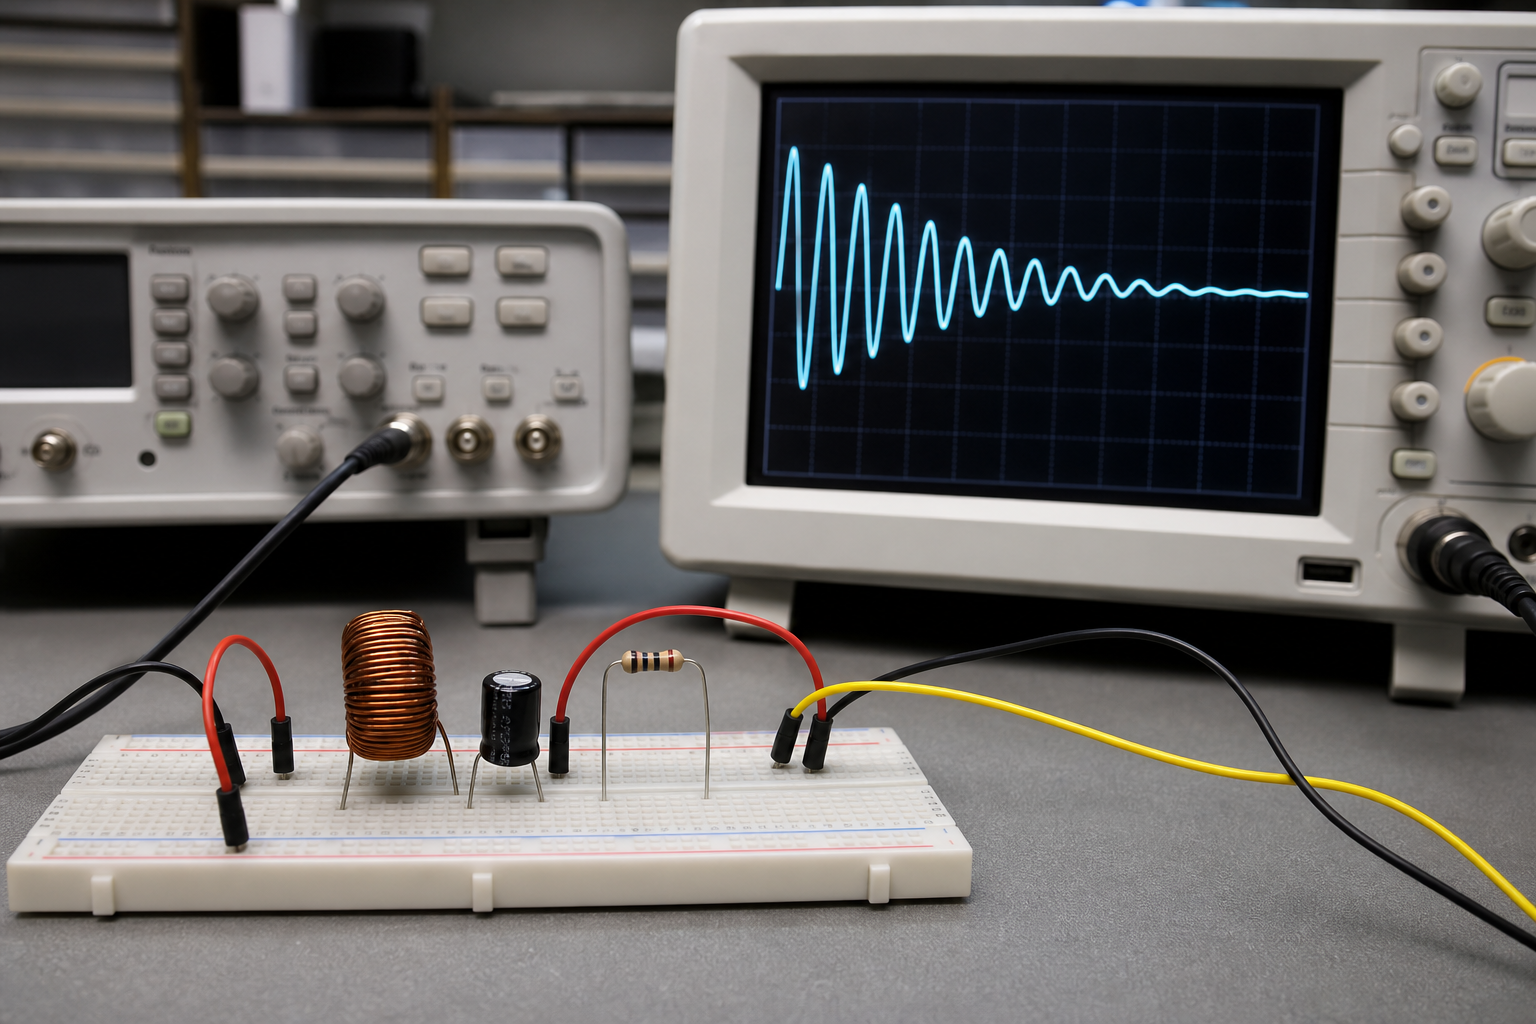
\includegraphics[width=0.60\linewidth]{images/book3/ai/b3-07-rlc-breadboard-oscilloscope.png}

{\small Een spoel, een condensator en een weerstand op een experimenteerbord, en op de oscilloscoop de uitdovende trilling die op een sprong volgt: het \omterm{thm:b1:transient-regimes:regimes}{pseudoperiodieke regime} van dit hoofdstuk.}
\end{omfigure}

\section{Systemen van de eerste orde}

\begin{definition}[Lineair systeem van de eerste orde]\label{def:b1:transient-regimes:firstorder}
\index{systeem van de eerste orde}\index{tijdconstante}\index{overgangsverschijnsel}\index{eindtoestand}
Een grootheid $x(t)$ voldoet aan een \emph{lineaire eerste-ordevergelijking
met constante coëfficiënten} wanneer
\[
\tau\,\frac{\dd x}{\dd t} + x = x_\infty ,
\]
met $\tau > 0$ de \emph{tijdconstante} en $x_\infty$ een constante (de
waarde die de bron oplegt). Haar \emph{eindtoestand} is $x = x_\infty$;
het \emph{overgangsverschijnsel} is de weg daarheen vanaf de beginwaarde
$x(0) = x_0$.
\end{definition}

\begin{theorem}[Oplossing]\label{thm:b1:transient-regimes:firstorder}
De enige oplossing met $x(0) = x_0$ is
\[
x(t) = x_\infty + (x_0 - x_\infty)\,\eu^{-t/\tau} .
\]
Het gat tot de \omterm{def:b1:transient-regimes:firstorder}{eindtoestand} krimpt met de factor $\eu^{-1} \approx
0.37$ per $\tau$: $63\%$ van de weg na $\tau$, $95\%$ na $3\tau$,
$99\%$ na $4.6\tau$. De raaklijn in de oorsprong bereikt $x_\infty$ op
$t = \tau$.
\end{theorem}

\begin{proof}
$y = x - x_\infty$ voldoet aan $\tau y' + y = 0$, waarvan de oplossingen
$y = K\eu^{-t/\tau}$ zijn (de wiskunde over lineaire
differentiaalvergelijkingen bewijst dat er geen andere zijn); $K = x_0 - x_\infty$. De helling
in $0$ is $-(x_0 - x_\infty)/\tau$, die het gat in de tijd
$\tau$ zou dichten.
\end{proof}

\begin{omfigure}
\begin{tikzpicture}
\begin{axis}[omaxis, width=9.4cm, height=5.4cm, xlabel={$t$}, ylabel={$x$},
    xmin=0, xmax=5, ymin=0, ymax=1.35, xtick={1,2,3,4,5},
    xticklabels={$\tau$,$2\tau$,$3\tau$,$4\tau$,$5\tau$},
    ytick={0.632,1}, yticklabels={$0.63$,$x_\infty$}]
  \addplot[omExo, dashed, domain=0:5, samples=2] {1};
  \addplot[omExo, dashed, domain=0:1, samples=2] {x};
  \addplot[omDef, thick, domain=0:5, samples=100] {1 - exp(-x)};
  \draw[dashed, omExo] (axis cs:1,0) -- (axis cs:1,0.632) -- (axis cs:0,0.632);
  \draw[dashed, omExo] (axis cs:3,0) -- (axis cs:3,0.95);
  \node[omExo, below right, font=\footnotesize] at (axis cs:3,0.95) {$0.95\,x_\infty$};
  \node[omDef, font=\footnotesize, below right] at (axis cs:2.2,0.75) {$x_\infty(1 - \eu^{-t/\tau})$};
\end{axis}
\end{tikzpicture}

{\small Het eerste-ordeantwoord op een sprong vanuit $x_0 = 0$: de
raaklijn in de oorsprong snijdt de asymptoot op $t = \tau$; $63\%$ van de weg na $\tau$,
$95\%$ na $3\tau$. Elk eerste-orde-overgangsverschijnsel is deze kromme, uitgerekt
met $\tau$ en verschoven met $x_0$ en $x_\infty$.}
\end{omfigure}

\begin{proposition}[RC- en RL-kringen]\label{prop:b1:transient-regimes:rcrl}
\index{RC-kring}\index{RL-kring}
Een condensator $C$ die via een weerstand $R$ vanuit een ideale bron $E$ wordt
geladen voldoet aan $RC\,\dd u_C/\dd t + u_C = E$: $\tau = RC$, $u_{C,\infty} = E$. Een
spoel $L$ in serie met $R$ over $E$ voldoet aan $(L/R)\,\dd i/\dd t + i =
E/R$: $\tau = L/R$, $i_\infty = E/R$. Met de bron weggenomen
($E \to 0$) beschrijven dezelfde vergelijkingen de ontlading naar nul.
\end{proposition}

\begin{proof}
Maasregel $E = Ri + u_C$ met $i = C\,\dd u_C/\dd t$; maasregel
$E = Ri + L\,\dd i/\dd t$.
\end{proof}

\begin{proposition}[Continuïteitsvoorwaarden]\label{prop:b1:transient-regimes:continuity}
\index{continuïteit (van $u_C$, van $i_L$)}
De \omterm{def:b1:dc-circuits:voltage}{spanning} over een condensator en de stroom door een spoel zijn
continue functies van de tijd: op een schakelmoment $t_0$ geldt
$u_C(t_0^+) = u_C(t_0^-)$ en $i_L(t_0^+) = i_L(t_0^-)$. Stromen door
weerstanden en \omterm{def:b1:dc-circuits:voltage}{spanningen} over spoelen mogen springen.
\end{proposition}

\begin{proof}
Een sprong van $u_C$ zou een oneindige $i = C\,\dd u_C/\dd t$ vergen, een sprong
van $i_L$ een oneindige $u = L\,\dd i/\dd t$; beide zijn
onmogelijk in een kring met eindige \omterm{def:b1:dc-circuits:voltage}{spanningen} en stromen (evenzo kunnen
de opgeslagen energieën $\tfrac12 Cu_C^2$ en $\tfrac12 Li^2$ niet
ogenblikkelijk veranderen zonder oneindig vermogen).
\end{proof}

\begin{method}[Een eerste-orde-overgang oplossen]\label{met:b1:transient-regimes:first}
\begin{enumerate}
  \item Schrijf na de schakelaar de maas- en knooppuntregels op, met de
        componentwetten; herleid tot één vergelijking in $u_C$ of $i_L$ en
        breng haar in de vorm $\tau x' + x = x_\infty$; lees $\tau$ en
        $x_\infty$ af (het laatste is ook de \omterm{def:b1:transient-regimes:firstorder}{eindtoestand} die men vindt door
        $C$ door een open keten en $L$ door een draad te vervangen).
  \item Bepaal $x_0$ uit de continuïteit van $u_C$ of $i_L$ over het
        schakelmoment heen, met de kring \emph{ervóór}.
  \item Schrijf $x = x_\infty + (x_0 - x_\infty)\eu^{-t/\tau}$; leid
        de overige grootheden af door differentiëren en met de maasregel.
\end{enumerate}
Ziet de condensator een netwerk van weerstanden en bronnen, vervang dat
netwerk dan eerst door zijn Thévenin-equivalent $(E_{\mathrm{Th}}, R_{\mathrm{Th}})$
(\cref{ch:b1:dc-circuits}): $\tau = R_{\mathrm{Th}}C$,
$u_\infty = E_{\mathrm{Th}}$.
\end{method}

\begin{proposition}[Energiebalans van de RC-lading]\label{prop:b1:transient-regimes:rcenergy}
Bij het laden van een condensator van $0$ tot $E$ door een willekeurige weerstand $R$ levert de
bron $CE^2$, slaat de condensator $\tfrac12 CE^2$ op en dissipeert de
weerstand de andere $\tfrac12 CE^2$ --- wat $R$ ook is.
\end{proposition}

\begin{proof}
$i = (E/R)\eu^{-t/\tau}$; de bron levert $\int_0^\infty Ei\,\dd t
= E \cdot (E/R)\tau = CE^2$; de weerstand neemt $\int_0^\infty Ri^2\,\dd t
= (E^2/R)\int_0^\infty \eu^{-2t/\tau}\dd t = (E^2/R)(\tau/2) = \tfrac12 CE^2$;
het verschil is de opgeslagen $\tfrac12 CE^2$. Een kleinere $R$ dissipeert
dezelfde energie sneller.
\end{proof}

\begin{example}[Een relaisspoel]\label{ex:b1:transient-regimes:relay}
$L = \qty{20}{mH}$, $R = \qty{5.0}{\ohm}$, $E = \qty{10}{V}$: $\tau =
\qty{4.0}{ms}$, $i_\infty = \qty{2.0}{A}$; de contacten trekken aan wanneer
$i$ \qty{1.5}{A} bereikt, dus op $t = -\tau\ln(1 - 0.75) =
\qty{5.5}{ms}$. Bij het openen van de kring moet $i$ van \qty{2}{A} dalen; een
vrijloopdiode over de spoel geeft de stroom een weg door $R$
alleen, $\tau = \qty{4}{ms}$, in plaats van een vonk.
\end{example}

\section{Systemen van de tweede orde}

\begin{definition}[Canonieke tweede-ordevorm]\label{def:b1:transient-regimes:secondorder}
\index{systeem van de tweede orde}\index{eigenhoekfrequentie}\index{kwaliteitsfactor}\index{dempingsverhouding}
Een grootheid $x(t)$ vormt een \emph{lineair systeem van de tweede orde} wanneer
\[
\frac{\dd^2 x}{\dd t^2} + \frac{\omega_0}{Q}\,\frac{\dd x}{\dd t} + \omega_0^2\,x
= \omega_0^2\,x_\infty ,
\]
met $\omega_0 > 0$ de \emph{eigenhoekfrequentie}, $Q > 0$ de
\emph{kwaliteitsfactor} (\omterm{def:b1:units-dimensions:dimension}{dimensieloos}) en $x_\infty$ de \omterm{def:b1:transient-regimes:firstorder}{eindtoestand}.
Men schrijft ook $\omega_0/Q = 2\xi\omega_0$ met $\xi = 1/2Q$ de
\emph{dempingsverhouding}.
\end{definition}

\begin{proposition}[De RLC-kring in serie]\label{prop:b1:transient-regimes:rlc}
\index{RLC-kring}
Een condensator $C$, een spoel $L$ en een weerstand $R$ in serie over een bron
$E$: de \omterm{def:b1:dc-circuits:voltage}{spanning} over de condensator voldoet aan de canonieke vorm met
\[
\omega_0 = \frac{1}{\sqrt{LC}}, \qquad Q = \frac{1}{R}\sqrt{\frac{L}{C}},
\qquad u_{C,\infty} = E .
\]
\end{proposition}

\begin{proof}
Maasregel: $E = L\,\dd i/\dd t + Ri + u_C$ met $i = C\,\dd u_C/\dd t$:
$LC\,u_C'' + RC\,u_C' + u_C = E$; deel door $LC$ en identificeer
$\omega_0^2 = 1/LC$, $\omega_0/Q = R/L$.
\end{proof}

\begin{omfigure}
\begin{tikzpicture}[font=\small]
  \draw (0,0) to[battery1, l=$E$, invert] (0,2.6) to[R=$R$] (2.4,2.6) to[L=$L$, i=$i$] (4.8,2.6) -- (4.8,2.6) to[C=$C$, v=$u_C$] (4.8,0) -- (0,0);
  \begin{scope}[xshift=7.6cm]
    \draw[thick] (0,0) -- (0,3.4);
    \fill[pattern=north east lines] (-0.25,0) rectangle (0,3.4);
    % spring
    \draw[thick] (0,2.6) -- (0.4,2.6) \foreach \i in {0,...,5} {-- ++(0.2,0.25) -- ++(0.2,-0.5) -- ++(0.2,0.25)} -- (3.3,2.6);
    % damper
    \draw[thick] (0,0.8) -- (1.2,0.8);
    \draw[thick] (1.2,0.5) -- (1.2,1.1) -- (2.2,1.1); \draw[thick] (1.2,0.5) -- (2.2,0.5);
    \draw[thick] (1.9,0.6) -- (1.9,1.0); \draw[thick] (1.9,0.8) -- (3.3,0.8);
    \draw[thick, fill=omDef!15] (3.3,0.2) rectangle (4.5,3.2); \node at (3.9,1.7) {$m$};
    \draw[-Stealth] (3.9,3.5) -- (5.2,3.5) node[right] {$x$};
    \node at (1.7,3.15) {$k$}; \node at (1.7,0.1) {$\alpha$};
  \end{scope}
\end{tikzpicture}

{\small De twee gezichten van het tweede-ordesysteem: de \omterm{prop:b1:transient-regimes:rlc}{RLC-kring} in
serie ($\omega_0 = 1/\sqrt{LC}$, $Q = \sqrt{L/C}/R$) en het stelsel
massa--veer--demper ($\omega_0 = \sqrt{k/m}$, $Q = \sqrt{km}/\alpha$).
Dezelfde vergelijking, dezelfde drie regimes.}
\end{omfigure}

\begin{proposition}[De mechanische oscillator]\label{prop:b1:transient-regimes:mechanical}
\index{massa--veer--demper}\index{elektromechanische analogie}
Een massa $m$ aan een veer met veerconstante $k$ met een viskeuze demper met
coëfficiënt $\alpha$ (kracht $-\alpha\dot x$), over $x$ uit het evenwicht
verplaatst, voldoet aan $m\ddot x + \alpha\dot x + kx = 0$: de canonieke vorm
met
\[
\omega_0 = \sqrt{\frac{k}{m}}, \qquad Q = \frac{\sqrt{km}}{\alpha} .
\]
De overeenkomst $x \leftrightarrow q$, $\dot x \leftrightarrow i$,
$m \leftrightarrow L$, $\alpha \leftrightarrow R$, $k \leftrightarrow 1/C$
beeldt elk resultaat van het ene systeem op het andere af.
\end{proposition}

\begin{proof}
De tweede wet van Newton (\cref{ch:b1:newton-dynamics}) met de veerkracht
$-kx$ en de dempingskracht; deel door $m$.
\end{proof}

\begin{theorem}[De drie regimes]\label{thm:b1:transient-regimes:regimes}
\index{aperiodisch regime}\index{kritisch regime}\index{pseudoperiodiek regime}\index{pseudoperiode}
De oplossingen van de homogene vergelijking $x'' + (\omega_0/Q)x' +
\omega_0^2 x = 0$ worden beheerst door de wortels van $r^2 + (\omega_0/Q)r +
\omega_0^2 = 0$, met discriminant $\Delta = \omega_0^2(1/Q^2 - 4)$:
\begin{itemize}
  \item $Q < \tfrac12$, \emph{aperiodisch}: twee reële negatieve wortels
        $r_\pm = -\frac{\omega_0}{2Q}\big(1 \mp \sqrt{1 - 4Q^2}\big)$,
        $x = A\eu^{r_+t} + B\eu^{r_-t}$, een terugkeer zonder trilling;
  \item $Q = \tfrac12$, \emph{kritisch}: een dubbele wortel $r = -\omega_0$,
        $x = (A + Bt)\eu^{-\omega_0 t}$, de snelste terugkeer zonder
        doorschot;
  \item $Q > \tfrac12$, \emph{pseudoperiodiek}: complexe wortels
        $r = -1/\tau \pm \iu\omega$ met
        \[
        \tau = \frac{2Q}{\omega_0}, \qquad
        \omega = \omega_0\sqrt{1 - \frac{1}{4Q^2}},
        \qquad
        x = \eu^{-t/\tau}\big(A\cos\omega t + B\sin\omega t\big),
        \]
        een gedempte trilling met \emph{pseudoperiode} $T = 2\pi/\omega$
        binnen de omhullende $\pm\sqrt{A^2 + B^2}\,\eu^{-t/\tau}$.
\end{itemize}
De volledige oplossing bij een constant rechterlid is $x_\infty$ plus de
homogene oplossing; $A$ en $B$ volgen uit $x(0)$ en $x'(0)$.
\end{theorem}

\begin{proof}
De karakteristieke vergelijking van een lineaire vergelijking met vaste
coëfficiënten (wiskunde, lineaire vergelijkingen van de tweede orde): de
wortels zijn $r = -\omega_0/2Q \pm \tfrac12\sqrt\Delta$. Voor $Q > \tfrac12$ is
$\sqrt\Delta = \iu\omega_0\sqrt{4 - 1/Q^2}$, wat het reële deel
$-\omega_0/2Q = -1/\tau$ en het imaginaire deel $\pm\omega_0\sqrt{1 - 1/4Q^2}$ geeft;
de reële oplossingen zijn de combinaties van $\eu^{-t/\tau}\cos\omega t$
en $\eu^{-t/\tau}\sin\omega t$.
\end{proof}

\begin{omfigure}
\begin{tikzpicture}
\begin{axis}[omaxis, width=11.5cm, height=6cm, xlabel={$\omega_0 t$}, ylabel={$x/x_\infty$},
    xmin=0, xmax=16, ymin=0, ymax=1.75, xtick={0,5,10,15}, ytick={0.5,1,1.5},
    legend style={at={(0.97,0.97)}, anchor=north east, font=\footnotesize, draw=none, fill=none}]
  % Q=0.2: roots r = -(1/(2Q))(1 -/+ sqrt(1-4Q^2)) = -2.5(1 -/+ 0.6) = -1, -4 ; x = 1 - (4 e^{-t} - e^{-4t})/3
  \addplot[omProp, thick, domain=0:16, samples=200] {1 - (4*exp(-x) - exp(-4*x))/3};
  \addlegendentry{$Q = 0.2$ (aperiodisch)}
  \addplot[omThm, thick, domain=0:16, samples=200] {1 - (1 + x)*exp(-x)};
  \addlegendentry{$Q = 0.5$ (kritisch)}
  % Q=3: tau=6, w = sqrt(1-1/36)=0.986 ; x = 1 - e^{-t/6}(cos wt + sin wt /(6 w))
  \addplot[omDef, thick, domain=0:16, samples=400] {1 - exp(-x/6)*(cos(deg(0.986*x)) + sin(deg(0.986*x))/(6*0.986))};
  \addlegendentry{$Q = 3$ (pseudoperiodiek)}
  \addplot[omExo, dashed, domain=0:16, samples=2] {1};
\end{axis}
\end{tikzpicture}

{\small Antwoord op een sprong vanuit rust van een tweede-ordesysteem, voor drie
\omterm{def:b1:transient-regimes:secondorder}{kwaliteitsfactoren}. Kleine $Q$: een traag kruipen; $Q = \tfrac12$: de snelste
terugkeer zonder doorschot; grote $Q$: naklank die ongeveer $Q$
trillingen duurt.}
\end{omfigure}

\begin{proposition}[$Q$ aflezen op een pseudoperiodiek beeld]\label{prop:b1:transient-regimes:decrement}
\index{logaritmisch decrement}
In het \omterm{thm:b1:transient-regimes:regimes}{pseudoperiodieke regime} staan twee opeenvolgende maxima in de verhouding
$x_{n+1}/x_n = \eu^{-T/\tau}$; het \emph{\omterm{prop:b1:transient-regimes:decrement}{logaritmisch decrement}}
\[
\delta = \ln\frac{x_n}{x_{n+1}} = \frac{T}{\tau} = \frac{\pi}{Q\sqrt{1 - 1/4Q^2}}
\approx \frac{\pi}{Q} \quad (Q \gg 1)
\]
geeft $Q$; het aantal trillingen dat zichtbaar is voordat de \omterm{def:b1:wave-propagation:signal}{amplitude}
onder $5\%$ zakt is ongeveer $Q$. Voor $Q \gg 1$ is $\omega \approx \omega_0$
en $T \approx 2\pi/\omega_0$.
\end{proposition}

\begin{proof}
De omhullende $\eu^{-t/\tau}$ wordt per periode met $\eu^{-T/\tau}$ vermenigvuldigd;
$T/\tau = (2\pi/\omega)(\omega_0/2Q)$. De omhullende bereikt $\eu^{-3}
\approx 5\%$ op $3\tau = 6Q/\omega_0 \approx Q\,T$, dus na ongeveer
$Q$ perioden.
\end{proof}

\begin{omfigure}
\begin{tikzpicture}
\begin{axis}[omaxis, width=11.5cm, height=5.6cm, xlabel={$t$}, ylabel={$x$},
    xmin=0, xmax=12.5, ymin=-1.2, ymax=1.3, xtick={2,4,6,8,10,12},
    xticklabels={$T$,$2T$,$3T$,$4T$,$5T$,$6T$}, ytick={-1,1}, yticklabels={$-x_0$,$x_0$}]
  \addplot[omExo, dashed, domain=0:12.5, samples=60] {exp(-x/5)};
  \addplot[omExo, dashed, domain=0:12.5, samples=60] {-exp(-x/5)};
  \addplot[omDef, thick, domain=0:12.5, samples=500] {exp(-x/5)*cos(deg(pi*x))};
  \fill[omThm] (axis cs:0,1) circle (1.4pt) node[above right, font=\footnotesize] {$x_0$};
  \fill[omThm] (axis cs:2,0.670) circle (1.4pt) node[above right, xshift=2pt, yshift=3pt, font=\footnotesize] {$x_1 = x_0\eu^{-T/\tau}$};
  \fill[omThm] (axis cs:4,0.449) circle (1.4pt) node[above right, xshift=2pt, yshift=3pt, font=\footnotesize] {$x_2$};
\end{axis}
\end{tikzpicture}

{\small Vrije pseudoperiodieke uitdemping, $x = x_0\eu^{-t/\tau}\cos\omega t$:
opeenvolgende maxima krimpen met de constante factor $\eu^{-T/\tau}$, en
$\ln(x_n/x_{n+1}) = T/\tau \approx \pi/Q$ meet de \omterm{def:b1:transient-regimes:secondorder}{kwaliteitsfactor}
van het beeld af.}
\end{omfigure}

\begin{example}[Een RLC-naklank]\label{ex:b1:transient-regimes:rlcnum}
$L = \qty{10}{mH}$, $C = \qty{100}{nF}$, $R = \qty{100}{\ohm}$:
$\omega_0 = 1/\sqrt{10^{-9}} = \qty{3.16e4}{rad/s}$ ($f_0 =
\qty{5.03}{kHz}$), $Q = \sqrt{L/C}/R = 316/100 = 3.16$: pseudoperiodiek,
$\tau = 2Q/\omega_0 = \qty{0.20}{ms}$, $\omega = 0.987\,\omega_0$,
$T = \qty{0.20}{ms}$, drie zichtbare trillingen. De kritische weerstand
is $R_c = 2\sqrt{L/C} = \qty{632}{\ohm}$; daarboven is de ontlading
aperiodisch.
\end{example}

\begin{method}[Een tweede-orde-overgang oplossen]\label{met:b1:transient-regimes:second}
\begin{enumerate}
  \item Schrijf de vergelijking op; breng haar in canonieke vorm; lees $\omega_0$,
        $Q$ en $x_\infty$ af.
  \item Bepaal het regime uit $Q$ en schrijf de algemene oplossing als
        $x_\infty$ plus de homogene oplossing.
  \item Bepaal $x(0)$ en $x'(0)$ uit de continuïteit van $u_C$ en $i_L$
        (voor de RLC: $u_C(0^+) = u_C(0^-)$ en $u_C'(0^+) = i(0^-)/C$);
        los de twee constanten op.
\end{enumerate}
\end{method}

\begin{example}[Beginvoorwaarden]\label{ex:b1:transient-regimes:ic}
De condensator uit het vorige voorbeeld is tot $U_0$ geladen en wordt op
$t = 0$ op $L$ en $R$ gesloten (geen bron): $x_\infty = 0$,
$u_C(0) = U_0$, $u_C'(0) = i(0)/C = 0$, want de spoelstroom was nul.
Dus $A = U_0$ en $-A/\tau + B\omega = 0$, $B = U_0/(\omega\tau) =
U_0/\sqrt{4Q^2 - 1}$: $u_C = U_0\eu^{-t/\tau}[\cos\omega t + \sin(\omega
t)/\sqrt{4Q^2 - 1}]$ --- voor $Q \gg 1$ eenvoudig $U_0\eu^{-t/\tau}\cos\omega_0 t$,
en de stroom $i = -C\,\dd u_C/\dd t$ piekt rond $U_0\sqrt{C/L} =
U_0/(\omega_0 L)$.
\end{example}

\begin{remark}[Energie]\label{rem:b1:transient-regimes:energy}
De opgeslagen energie $\tfrac12 Cu_C^2 + \tfrac12 Li^2$ (of $\tfrac12 kx^2
+ \tfrac12 m\dot x^2$) neemt af met de snelheid $Ri^2$ ($\alpha\dot x^2$):
differentieer en gebruik de vergelijking. Per pseudoperiode krimpt de energie
met de factor $\eu^{-2T/\tau}$; bij $Q = 3$ gaat ongeveer $88\%$ ervan
verloren per trilling. Een hoge $Q$ betekent een traag lek ten opzichte van de
trilling --- een goede klok, een scherpe resonantie
(\cref{ch:b1:sinusoidal-impedance}) --- en een lage $Q$ een snelle terugkeer:
de juiste keuze voor een vering of een meternaald.
\end{remark}

\section{Oefeningen}

\begin{exercise}[$\star$]\label{exo:b1:transient-regimes:1}
Een \omterm{prop:b1:transient-regimes:rcrl}{RC-kring}: $R = \qty{10}{k\ohm}$, $C = \qty{47}{nF}$, geladen vanuit
$E$. Bereken $\tau$, $u_C(\tau)/E$ en de tijd om $99\%$ van $E$ te bereiken.
\end{exercise}

\begin{exercise}[$\star$]\label{exo:b1:transient-regimes:2}
Een \omterm{prop:b1:transient-regimes:rcrl}{RL-kring}: $L = \qty{20}{mH}$, $R = \qty{5.0}{\ohm}$, $E = \qty{10}{V}$.
Bereken $\tau$, de eindstroom, de stroom op $t = \tau$ en de
\omterm{def:b1:dc-circuits:voltage}{spanning} over de spoel vlak na het sluiten van de schakelaar.
\end{exercise}

\begin{exercise}[$\star$]\label{exo:b1:transient-regimes:3}
Een RLC in serie: $L = \qty{10}{mH}$, $C = \qty{100}{nF}$, $R = \qty{100}{\ohm}$.
Bereken $\omega_0$, $f_0$, $Q$; benoem het regime; geef $\tau$ en de
pseudoperiode.
\end{exercise}

\begin{exercise}[$\star$]\label{exo:b1:transient-regimes:4}
Welke weerstand geeft bij dezelfde $L$ en $C$ het \omterm{thm:b1:transient-regimes:regimes}{kritische regime}?
Wat is $Q$ dan? Wat gebeurt er voor $R = \qty{2}{k\ohm}$?
\end{exercise}

\begin{exercise}[$\star\star$]\label{exo:b1:transient-regimes:5}
Een geladen condensator $C = \qty{1.0}{\micro F}$ ontlaadt zich over een
onbekende $R$; de \omterm{def:b1:dc-circuits:voltage}{spanning} halveert elke \qty{3.5}{ms}. Toon aan dat de
halveringstijd $\tau\ln 2$ is en bepaal $R$.
\end{exercise}

\begin{exercise}[$\star\star$]\label{exo:b1:transient-regimes:6}
Toon door directe integratie aan dat het laden van een condensator van $0$ tot $E$
via $R$ precies $\tfrac12 CE^2$ in $R$ dissipeert, onafhankelijk van
$R$. Wat wordt daarmee het rendement van de overdracht, en hoe zou het
beter kunnen?
\end{exercise}

\begin{exercise}[$\star\star$]\label{exo:b1:transient-regimes:7}
Op een oscilloscoop toont een vrije RLC-uitdemping opeenvolgende maxima van
\qty{2.0}{V}, \qty{1.5}{V}, \qty{1.12}{V} met tussenpozen van \qty{0.40}{ms}.
Leid $Q$ en $\omega_0$ af, en met $C = \qty{1.0}{\micro F}$ de waarden
van $L$ en $R$.
\end{exercise}

\begin{exercise}[$\star\star$]\label{exo:b1:transient-regimes:8}
Een condensator geladen tot $U_0 = \qty{100}{V}$ ($C = \qty{10}{\micro F}$) wordt
op een spoel $L = \qty{1.0}{mH}$ met kleine weerstand geschakeld ($Q \gg 1$).
Schrijf $u_C(t)$ en $i(t)$ op en schat de piekstroom. Waar zit
de energie op het moment van de piek?
\end{exercise}

\begin{exercise}[$\star\star$]\label{exo:b1:transient-regimes:9}
Een kwart auto: $m = \qty{400}{kg}$ op een veer $k = \qty{2.0e4}{N/m}$.
Bereken $\omega_0$, $f_0$ en de kritische dempingscoëfficiënt. Geef met een
demper $\alpha = \qty{2000}{N.s/m}$ de waarde van $Q$, het regime, de
pseudoperiode en de uitdooftijd $\tau$.
\end{exercise}

\begin{exercise}[$\star\star\star$]\label{exo:b1:transient-regimes:10}
Een spoel $L = \qty{0.50}{H}$ voert $I_0 = \qty{2.0}{A}$; de bron wordt
losgekoppeld en de spoel blijft op een ontlaadweerstand $R = \qty{100}{\ohm}$ staan.
Geef $i(t)$, $\tau$, de piekspanning over de spoel en de gedissipeerde
energie. Wat zou er zonder die weerstand gebeuren?
\end{exercise}

\begin{exercise}[$\star\star\star$]\label{exo:b1:transient-regimes:11}
Een condensator $C = \qty{1.0}{\micro F}$ wordt vanuit $E = \qty{12}{V}$
geladen via $R_1 = \qty{10}{k\ohm}$, terwijl $R_2 = \qty{20}{k\ohm}$ er
overheen staat. Bepaal met een Thévenin-equivalent de \omterm{def:b1:transient-regimes:firstorder}{tijdconstante} en de
eindspanning; schrijf $u_C(t)$ op vanaf $u_C(0) = 0$.
\end{exercise}

\begin{exercise}[$\star\star\star$]\label{exo:b1:transient-regimes:12}
\omterm{thm:b1:transient-regimes:regimes}{Kritisch regime}, sprong vanuit rust ($x(0) = x'(0) = 0$): toon aan dat
$x = x_\infty[1 - (1 + \omega_0 t)\eu^{-\omega_0 t}]$, en bepaal
numeriek de tijd om $95\%$ van $x_\infty$ te bereiken (in eenheden van
$1/\omega_0$). Vergelijk met de insteltijd van de omhullende voor $Q = 5$
en met die van de trage wortel voor $Q = 0.1$; concludeer waarom ``kritisch'' het
doel van de ingenieur is.
\end{exercise}

\section{Probleem: Een vering ontwerpen}

\begin{problem}[{Weekendopgave --- dezelfde differentiaalvergelijking op
een labtafel en onder een auto: hoeveel keer een versleten schokdemper laat
wippen, wat de ontwerper in plaats daarvan kiest, en hoe één getal
de twee uit elkaar houdt}]
\label{pb:b1:transient-regimes:1}
Deel I bestudeert een \omterm{prop:b1:transient-regimes:rlc}{RLC-kring} in serie, $L = \qty{10}{mH}$, $C = \qty{100}{nF}$;
de delen II--IV een kwartautomodel: een massa $m = \qty{350}{kg}$ rustend op een
veer $k = \qty{22}{kN/m}$ met een schokdemper die $-\alpha\dot x$ uitoefent.
Het doorschot van een sprongantwoord in het \omterm{thm:b1:transient-regimes:regimes}{pseudoperiodieke regime} (gegeven):
$x_{\max}/x_\infty - 1 = \exp(-\pi\xi/\sqrt{1 - \xi^2})$, $\xi = 1/2Q$.

\medskip
\noindent\textbf{Deel I --- De schakeling.}
\begin{enumerate}
  \item Schrijf de maasregel op voor de RLC in serie over een bron $E$, en
        de differentiaalvergelijking voor $u_C$.
  \item Breng haar in canonieke vorm; druk $\omega_0$ en $Q$ uit.
  \item Bereken $\omega_0$, $f_0$ en de kritische weerstand $R_c$.
  \item Schrijf de karakteristieke vergelijking en haar discriminant op; benoem
        de drie regimes in termen van $Q$.
  \item Geef in het pseudoperiodieke geval $\tau$ en $\omega$ en de
        vorm van $u_C(t)$.
  \item Bereken voor $R = \qty{100}{\ohm}$ de waarden van $Q$, $\tau$, de pseudoperiode
        en het aantal zichtbare trillingen.
  \item De condensator, tot $U_0$ geladen, wordt op $L$ en $R$ geschakeld
        op $t = 0$. Geef $u_C(0^+)$ en $\dd u_C/\dd t(0^+)$, met de
        natuurkundige reden voor elk.
\end{enumerate}

\medskip
\noindent\textbf{Deel II --- De kwartauto.}
\begin{enumerate}[resume]
  \item Meet $x$ vanaf de evenwichtsstand, schrijf de tweede wet van
        Newton voor de carrosserie op en toon aan dat het gewicht wegvalt.
  \item Breng de vergelijking in canonieke vorm; geef $\omega_0$ en $Q$ in
        termen van $m$, $k$, $\alpha$, en noem de elektromechanische
        overeenkomsten.
  \item Bereken $\omega_0$, $f_0$ en de kritische coëfficiënt
        $\alpha_c$.
  \item De ontwerper monteert $\alpha = \qty{4000}{N.s/m}$: bereken $Q$ en
        $\xi$, en benoem het regime.
  \item Bereken $\tau$ en de pseudoperiode.
  \item Bereken het doorschot na een sprong (een stoeprand): is de auto
        comfortabel?
  \item Welke weerstand $R$ zou de schakeling van deel I dezelfde
        $Q$ geven als deze vering?
\end{enumerate}

\medskip
\noindent\textbf{Deel III --- De versleten demper.}
Er is olie weggelekt: $\alpha = \qty{1200}{N.s/m}$.
\begin{enumerate}[resume]
  \item Bereken $Q$, de pseudoperiode en $\tau$.
  \item Met welke factor krimpen opeenvolgende maxima? Hoeveel keer wippen
        is zichtbaar voordat de \omterm{def:b1:wave-propagation:signal}{amplitude} onder $5\%$ zakt?
  \item De veertest: men duwt de hoek $x_0 =
        \qty{5.0}{cm}$ omlaag en laat los. Geef de beginvoorwaarden, de
        energie die in de veer is opgeslagen, en zeg waar die energie blijft.
  \item Schat de pieksnelheid van de carrosserie tijdens de eerste
        terugkeer ($\approx x_0\omega_0$ voor $Q \gg 1$) en de piekkracht in
        de demper.
  \item Waarom is precies kritische demping ($Q = \tfrac12$) niet de
        keuze van de ontwerper, hoewel zij geen doorschot geeft? (Denk aan
        de laatste millimeters van de terugkeer.)
  \item Bereken het doorschot voor de versleten demper en vergelijk met
        deel II.
\end{enumerate}

\medskip
\noindent\textbf{Deel IV --- $Q$ uit een beeld aflezen.}
Een versnellingsopnemer op de carrosserie registreert de vrije uitdemping.
\begin{enumerate}[resume]
  \item Voor de versleten auto zijn de opeenvolgende maxima $1.00$, $0.25$, $0.062$
        (willekeurige eenheden). Bereken het \omterm{prop:b1:transient-regimes:decrement}{logaritmisch decrement}, leid
        $\xi$ exact af uit $\delta = 2\pi\xi/\sqrt{1 - \xi^2}$ en daarna $Q$;
        vergelijk met deel III.
  \item Voor de gezonde auto is geen tweede maximum zichtbaar; alleen het
        doorschot, $3.8\%$, is af te lezen. Keer de doorschotformule om om
        $\xi$ en $Q$ te vinden.
  \item Welk deel van de mechanische energie dissipeert de versleten demper
        per pseudoperiode?
  \item Een monteur zonder auto bij de hand bouwt de RLC van deel I
        met een $R$ zo gekozen dat $Q = 2.3$: welke $R$, en waarom heeft het
        oscilloscoopbeeld, uitgezet tegen $\omega_0 t$, dezelfde vorm
        als dat van de auto?
  \item Vat samen: welk \omterm{def:b1:units-dimensions:dimension}{dimensieloos} getal de vorm van elk
        tweede-orde-overgangsverschijnsel bepaalt, welke waarde een ontwerper van
        een vering nastreeft, en wat een bestuurder moet afleiden uit ``meer dan
        één keer wippen''.
\end{enumerate}
\end{problem}
